%-----------------------------------------------------------------------------
%
%               Template for sigplanconf LaTeX Class
%
% Name:         sigplanconf-template.tex
%
% Purpose:      A template for sigplanconf.cls, which is a LaTeX 2e class
%               file for SIGPLAN conference proceedings.
%
% Guide:        Refer to "Author's Guide to the ACM SIGPLAN Class,"
%               sigplanconf-guide.pdf
%
% Author:       Paul C. Anagnostopoulos
%               Windfall Software
%               978 371-2316
%               paul@windfall.com
%
% Created:      15 February 2005
%
%-----------------------------------------------------------------------------


\documentclass[preprint,10pt,numbers]{sigplanconf}

% The following \documentclass options may be useful:

% preprint      Remove this option only once the paper is in final form.
% 10pt          To set in 10-point type instead of 9-point.
% 11pt          To set in 11-point type instead of 9-point.
% numbers       To obtain numeric citation style instead of author/year.

\usepackage{amsmath}

\newcommand{\cL}{{\cal L}}

% http://2016.onward-conference.org/home

\begin{document}

\special{papersize=8.5in,11in}
\setlength{\pdfpageheight}{\paperheight}
\setlength{\pdfpagewidth}{\paperwidth}

\conferenceinfo{CONF 'yy}{Month d--d, 20yy, City, ST, Country}
\copyrightyear{20yy}
\copyrightdata{978-1-nnnn-nnnn-n/yy/mm}
\copyrightdoi{nnnnnnn.nnnnnnn}

% Uncomment the publication rights you want to use.
%\publicationrights{transferred}
%\publicationrights{licensed}     % this is the default
%\publicationrights{author-pays}

\titlebanner{banner above paper title}        % These are ignored unless
\preprintfooter{short description of paper}   % 'preprint' option specified.

\title{Compressed Sensing as a Foundation for Software Testing}
%\subtitle{Subtitle Text, if any}

\authorinfo{Name1}
           {Affiliation1}
           {Email1}
\authorinfo{Name2\and Name3}
           {Affiliation2/3}
           {Email2/3}

\maketitle

\begin{abstract}
	Testing is perhaps the most popular way of ensuring software quality. Despite that, there are few principled methods to automatically test software, delta debugging being a notable exception. The gap that we address in this paper is how to efficiently test a software system under black-box assumptions with clearly articulated formal guarantees, where by efficiency we mean that only a small proportion of the overall test inputs is tried by the testing algorithm, and by formal guarantees we mean that the number of tests and probability of success follow from the testing framework.
	
	We address this challenge by making novel use of a technique from the area of signal processing known as \emph{compressed sensing}, and in particular its boolean variant known as \emph{group testing}. The key idea is to identify tests of interest by testing the system with random inputs that capture its input/output behavior, where group testing prescribes that tests are grouped together to minimize the number of inputs with a mathematical procedure how to recover single-element information from the results w.r.t. groups.
	
	As preliminary validation of the efficacy of compressed sensing in software testing, we report on experiments with web sanitizers and validators. The test inputs are cross-site scripting (XSS) payloads, and the output is a boolean indication whether or not the payloads penetrated through the built-in defenses. We demonstrate our ability to crack such defenses using only XXX tests, where brute-force testing would require XXX tests. This marks an XXX\% drop. 
\end{abstract}

\section{Introduction}

\begin{enumerate}
	\item background / motivation
	\item existing approaches
	\item our approach
	\item contributions
\end{enumerate}
\section{Motivation}
\section{Technical Overview}

We assume a finite alphabet $\Sigma=\{ \tau,\tau',\ldots \}$ of tokens used to express test inputs. An input is a member of $\Sigma^{\star}$. For example, input ${\sf <script>alert('1')</script>}$ consists of tokens ${\sf <script>}$, ${\sf alert('1')}$ and ${\sf </script>}$.

An \emph{element} is a token tuple, e.g. the 1-ary tuple ${\sf (<script>)}$ (or simply ${\sf <script>}$) or the 2-ary tuple ${\sf (<script>,</script>)}$. We say that input $i=\tau_1 \cdot \ldots \cdot \tau_n$ matches element $e$ or arity $k$, denoted $i \models e$, if
$$
\exists 1 \leq i_1 \leq \ldots \leq i_k \leq n.\ \bigwedge_{1 \leq m \leq k}
i(i_m) = e(m)  
$$
That is, the input contains a subsequence of tokens that matches the tokens specified as the element.

Input filtering (by which we refer collectively to both sanitization and validation) is modeled as a regular-expression membership judgment. This is, in fact, the common way of implementing such filters in practice \cite{XXX}. We follow the standard syntax for expressing a regular expression:
$$
	r = \epsilon\ |\ \{ \sigma \}_{\sigma \in \Sigma}\ |\ r + r\ |\ r \cdot r\ |\ r^{\star}
$$
For simplicity, and without loss of generality, we fix the behavior of the filter, such that given filter $r$ and input $i$, $i$ is in the language of $r$ --- denoted $i \in L_r$ --- iff $r$ \emph{rejects} $i$. That is, the filter matches against the input iff the input is considered illegal.

The problem we target in this paper is to characterize the behavior of a filter efficiently under black-box assumptions. Informally, what we mean by ``efficiently'' is that only a small fraction of the test inputs are tried. What we mean by ``black-box assumptions'' is that the testing system has no access to any of the code, and its behavior is based solely on the observed input/output pairs.




\section{The Theory of Compressed Sensing}

We now switch gears and focus on the theory of compressed sensing and group testing, which are the main mathematical tools we use for software testing. We first introduce the key concepts arising in compressed sensing: sparsity, linear measurements, and recovery of sparse active signals. We describe recoverability and efficient algorithms. We then move to Boolean compressed sensing, which is also known in statistics literature as the classical group testing problem \cite{dorfman1943detection, group_testing}. 


\subsection{Search for sparse signals}

There is a great variety of practical problems where we have an unknown vector $\bx$
of large dimensions $N$, which we would like to learn, but it is too expensive to measure all
the coordinates of the vector. The classical application which served as the original motivation
for group testing was testing US army recruits for syphilis during the Second World War. 
Individual blood tests for every one of the large number of recruits were too expensive, 
and statisticians consulting for the US army proposed to take pooled measurements, where 
each test was done on a mixture of blood samples coming from a number of carefully chosen subsets of recruits. Given enough such pooled tests, and assuming that only a small fraction of the recruits had the disease, it was possible to identify the infected recruits.  


In our application to security testing, there is a very large number of individual tokens and 
their small combinations such as pairs and triplets (or patterns as we refer to them). Testing each individual token, pair and 
triplet of tokens through a sanitizer is impractical -- requiring an immense number of calls to the 
sanitizer. However, we know that the vast majority of such patterns is innocuous, 
and only a very small fraction is malicious. 

Compressed sensing suggests to take a reduced set of aggregate measurements of the variable $\bx$,
where each measurement involves a subset of variables $x_i$ together.  For our application of
software testing we would create a string composed of multiple tokens of interest.  For the
army recruit testing problem one would mix the blood samples of multiple soldiers together
in one test-tube and administer the test on the mix.


Given these aggregate measurements where each variable $x_i$ may appear in multiple tests
(i.e., where each test involves a different but typically overlapping subset of indices), we would like to un-mix the
measurements to be able to precisely explain the anomalies at the level of individual tokens,
or individual sick soldiers.  The fact that this is at all possible may seem surprising, but it
is based on very elegant theory building on linear algebra and geometry of polytopes.  An
efficient solution is available using numerical optimization (namely linear programming) which
can recover the true identity of a sparse set of {\em active inputs} from a number of aggregate
measurements which is much smaller than $N$. Applications of similar flavor occur in
other diverse fields such as spectrum estimation, genetic disease testing, neuroscience, and even feature selection in machine learning \cite{rish2014sparse}. We next describe the mathematical foundations for this exciting theory.

\subsection{ Linear compressed sensing}

Suppose that  vector $\bx \in \rR^N$ has a small number $K$ of non-zero elements, $K \ll N$.
We denote the number of non-zero elements of $\bx$ using the $\ell_0$-norm notation:
$\Vert \bx \Vert_0 = K$.   We take $M$ aggregate linear measurements $y_i = \ba_i^T \bx$, where
$K < M \ll N$ and aggregate them into a vector $\by = [y_1, ..., y_M]$:
\begin{equation}
\by = A \bx,
\end{equation}
where the matrix $A$ contains vectors $\ba_i$ as rows. Now, given $\by$ and knowing the
measurement matrix $A$, can we hope to recover the unknown
sparse vector $\bx$?  It turns out that if $A$ was chosen properly, and if $\bx$ is sparse
enough, then indeed we can. Furthermore, this recovery can be done by an efficient optimization
procedure, namely linear programming (LP).

First we recall a theorem that allows brute force exact recovery \cite{donoho_pnas}. Define the {\em spark}
$S(A)$ of a matrix $A$ as the minimum number of linearly dependent columns of $A$. This is related to,
but different from rank of the matrix\footnote{For example, it's easy to construct a matrix of rank
$3$, which has two $2$ linearly dependent columns: just take an arbitrary rank-$3$ matrix and
copy one of the columns twice! This matrix has rank $3$ but it's spark is $2$. }. It turns out that
one can recover uniquely sparse vectors which have less than $S(A) / 2$ non-zero entries.

\begin{theorem}
970\label{thm:spark}
Suppose that $\Vert \bx \Vert_0 = K < S(A) / 2$. Then there is a unique solution to the
set of equations $\by = A \bx$.
\end{theorem}

This suggests that one can formulate the following optimization problem to find the sparse set of solutions
\begin{equation}
\label{eqn:l0_sparse_recovery}
\min_{\bx} \Vert \bx \Vert_0  ~~\mbox{ s.t. }~~ \by = A \bx
\end{equation}
Now, while the solution of this problem will give us the desired sparse signal (proviso the conditions in
theorem \ref{thm:spark}), the problem has no tractable solution; indeed it is an NP-hard problem \cite{natarajan1995sparse_recovery_complexity}. Astonishingly, under stronger conditions, the solution to this problem can be obtained exactly by a linear
programming (LP) relaxation where we replace the count of non-zeros $\Vert \bx \Vert_0$  by the $\ell_1$-norm
of the vector $\Vert \bx \Vert_1 = \sum_i | x_i|$. The problem becomes:\footnote{This optimization problem can be represented as a linear
program by a standard simple trick of introducing variables $\bx^+$ and $\bx^-$, where $\bx = \bx^+ - \bx^-$,
and $\bx^+, \bx^- \ge 0$. }
\begin{equation}
\label{eqn:l1_sparse_recovery}
\min_{\bx} \Vert \bx \Vert_1  ~~\mbox{ s.t. }~~ \by = A \bx
\end{equation}

The conditions in theorem \ref{thm:spark} are not sufficient to guarantee exact recovery of
sparse active inputs using the LP relaxation. However, let us define a relaxed notion of
well-posedness of the matrix $A$ called incoherence. Assume without loss of generality that
the columns of $A$ are normalized to have Euclidean unit norm, i.e., $\Vert A_i \Vert_2 = 1$.  We define the incoherence of $A$ to be:
\begin{equation}
M(A) \triangleq \max_{i \ne j} | A_i^T A_j |
\end{equation}
Using this definition, the following theorem holds:
\begin{theorem}
\label{thm:incoherence}
If $\Vert \bx \Vert_0 < \frac{ 1 + \frac{1}{M(A)}} {2}$ then the solution of the $\ell_1$-relaxed
problem (\ref{eqn:l1_sparse_recovery}) is also optimal for the combinatorial problem
(\ref{eqn:l0_sparse_recovery}).
\end{theorem}

Note that this does not mean that one can solve the NP-hard problem (\ref{eqn:l0_sparse_recovery})
using LP relaxations in general. This can be done only if the matrix is well-posed, as
specified by the incoherence condition, and if the signal of interest $\bx$ is sparse enough
with respect to $A$.

This condition is sufficient, but not the tightest known condition.
Stronger conditions have been developed based on the so-called Restricted Isometry Property,
\cite{candes2008_RIP} which considers larger subsets of columns of $A$, not just pairs.
However, verifying RIP is just as hard as solving problem (\ref{eqn:l0_sparse_recovery}) in general. In practice, RIP is used for random measurement
matrices $A$, which fortunately can be shown to satisfy the RIP property with high probability. \\


\section{ Boolean compressed sensing}
\label{s:boolean_compressed_sensing}
In many applications we have a very similar problem of having aggregate measurements
of a sparse unknown vector $\bx$, but the measurements may be non-linear.  For the application
to software testing, we will be especially interested in Boolean measurements, where the
vector $\bx$ is binary, and each measurement corresponds to a disjunction of a subset
of entries of $\bx$.  While one would think that recovery of active inputs from
Boolean measurements should be based on very different principles, it turns
out that the core information theoretic issues are closely related, and a very similar linear
programming relaxation can be used for recovery \cite{Malyutov78,MalioutovM2012}.

To set up the notation, we now assume that $\by$, $A$ and $\bx$ are all binary $\{0, 1\}$.
The boolean vector $\bx \in \{0, 1\}^N$, has $K \ll N$ non-zero (faulty) entries.
We will call items $j$ with $x_j = 0$ 'normal'. A pooled measurement $y_i$ is the
Boolean sum (Boolean OR) of $x_j$ in some subset $A_i \subset \{1,..,N\}$, i.e.,
\begin{equation}
y_i = \vee_{j \in A_i} x_j.
\end{equation}
The $M \times N$ measurement matrix $A$ satisfies $A_{ij} = 1$ if item $j$ belongs
to the subset pooled in test $i$. Other entries are $0$. We use the following vector
notation to describe the entire set of $M$ measurements:
\begin{equation*}
\by = A \vee \bx~~~~~~~~
\end{equation*}

\begin{figure}[!thb]
\centering
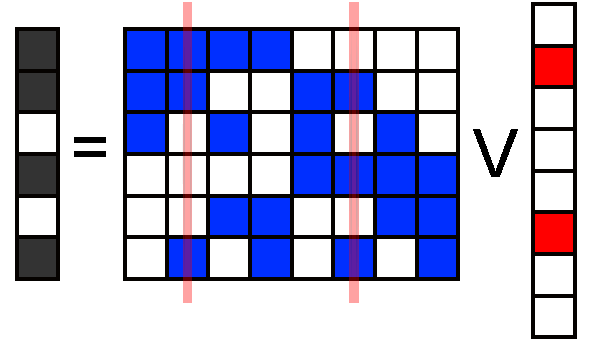
\includegraphics[width=1.5in]{./fig_group_test.pdf}
\caption{  Illustration of a pooled Boolean measurement.}
\label{fig:group_testing}
\end{figure}

It turns out that the story of exact recovery is parallel to the linear case:
if the matrix has well-distributed columns (as captured by the notion of disjunctness as 
defined below) and if the vector is sparse enough, then it can be uniquely recovered from the
Boolean measurements \cite{group_testing}.

\begin{definition}
We call a measurement matrix $\mathbf{A}$ {\em $K$-separating}
if all Boolean sums of subsets of $K$ columns are all distinct.
$\mathbf{A}$ is called {\em $K$-disjunct} if the union of any
$K$ columns does not contain any other column.
\end{definition}

Note that the $K$-separating property for $\mathbf{A}$ is sufficient
to allow exact recovery of $\mathbf{w}$ with up to $K$ nonzero entries
\cite{book2_group_testing}. However, finding the solution would
in general require searching over all $K$-subsets out of $N$. K-disjunctness
is a stronger condition, and allows the recovery using simpler algorithms.

The combinatorial algorithm asks to find the sparsest solution to the
set of Boolean equations which is done by solving the following optimization problem:
\begin{equation}
\label{eq:l0recovery}
	\min \|\mathbf{x}\|_0 \quad {\textrm{such that }}\mathbf{y} = \mathbf{A} \lor \mathbf{x},
\end{equation}

We now describe the LP relaxation for the Boolean sparse recovery problem. While
the problem in (\ref{eq:l0recovery}) looks very similar to the linear one in
(\ref{eqn:l0_sparse_recovery}), the key challenge is that the measurements are not linear. However, they can be represented equivalently by a pair of linear equalities and inequalities.

Let $\mP= \{i | y_i = 1\}$ be the set of measurements $i$ where $y_i$ is positive,
and $\mZ = \{i | y_i = 0\}$ be the set of zero (or negative) tests. Then we can
see that for $i \in \mZ$ we have
\begin{equation}
\mathbf{A}_{\mZ}\lor\mathbf{x} = \mathbf{0} ~~~\Leftrightarrow~~~ \mathbf{A}_{\mZ}\mathbf{x} = \mathbf{0}
\end{equation}
For the set of positive measurements, in the Boolean case $1\lor 1 = 1$, while
in the linear case $1 + 1 = 2$, but it is always true that
\begin{equation}
\mathbf{A}_{\mP}\lor\mathbf{x} =\mathbf{1} ~~~\Leftrightarrow~~~ \mathbf{A}_{\mP}\mathbf{x} \ge \mathbf{1}
\end{equation}
These constraints can be incorporated into an equivalent integer program (IP):
\begin{align}
\label{eq:booleanl1min}
	\min\quad &\sum_{j=1}^{n} x_j \\
	\textrm{s.t.\quad} & x_j \in \{0,1\},\,j = 1,\ldots,n\nonumber\\
		& \mathbf{A}_{\mP}\bx \ge \mathbf{1}\nonumber\\
		& \mathbf{A}_{\mZ}\bx = \mathbf{0}.\nonumber
\end{align}
Note that since $\bx$ is Boolean, the objectives in problems (\ref{eq:l0recovery}) and (\ref{eq:booleanl1min}) are equivalent (i.e., $\|x\|_0=\sum_i{x_i}$), and yet still, the problem
\eqref{eq:booleanl1min} is NP-hard because of the Boolean integer constraint on the weights. However, relaxing the binary constraints to linear interval constraints, we get a tractable linear program (LP):
\begin{align}
\label{eq:booleanl1minLP}
	\min\quad &\sum_{j=1}^{n} x_j \\
	\textrm{s.t.\quad} & 0\leq x_j \leq 1, \,j = 1,\ldots,n\nonumber\\
		& \mathbf{A}_{\mP}\bx \ge \mathbf{1}\nonumber\\
		& \mathbf{A}_{\mZ}\bx = \mathbf{0}.\nonumber
\end{align}

In \cite{MalioutovM2012} it was shown that if the $A$ matrix is $K$-disjunct, 
then we can recover sparse inputs $\bx$ with at most $K$ non-zero entries using 
the LP in (\ref{eq:booleanl1minLP}).
\begin{theorem}
\label{thm:LP_recovery}
Suppose there exists $\bx^*$ with $K$ nonzero entries and
$\by = \mathbf{A} \lor \bx^*$. If the matrix $\mathbf{A}$ is $K$-disjunct then
LP solution $\hat{\bx}$ in (\ref{eq:booleanl1minLP}) recovers $\bx^*$, i.e. $\hat{\bx} = \bx^*$.
\end{theorem}

This is a sufficient condition, but not necessary. In practice, one can often apply
the LP approach even if the LP yields fractional solution, with the help
of randomized rounding or other approaches for mapping to binary numbers.

In practical situations, we typically have noisy measurements.
We consider noise on the $\by$ vector, where some bits can flip from
$0$ to $1$ and vice versa. We represent this by
\begin{equation}
\label{eq:noisyforwardtest}
	\mathbf{y} = (\mathbf{A} \lor \mathbf{x}) \oplus \mathbf{n},
\end{equation}

To extend the LP formulation in the presence of noisy measurements (where $\mathbf{y} = (\mathbf{A} \lor \mathbf{x}) \oplus \mathbf{n}$), we look
for sparse rules that do not match $\by$ exactly, but rather approximate
$\by$ very closely. The corresponding LP formulation is:
\begin{align}
\label{eq:booleanl1minLPslack}
	\min\quad &\sum_{j=1}^{n} x_j + C\sum_{i=1}^{m}\xi_i\\
	\textrm{s.t.\quad} & 0 \le x_j \le 1,\,j = 1,\ldots,n\nonumber\\
		& 0 \le \xi_i \le 1, ~i \in \mP \nonumber\\
		& 0 \le \xi_i, ~i \in \mZ\nonumber\\
		& \mathbf{A}_{\mP}\mathbf{x} + \boldsymbol{\xi}_{\mP} \ge \mathbf{1}\nonumber\\
		& \mathbf{A}_{\mZ}\mathbf{x} = \boldsymbol{\xi}_{\mZ}.\nonumber
\end{align}
The regularization parameter $C$ trades off two objectives: minimizing the sparsity of $\bx$ versus minimizing a penalty on the number of errors in satisfying the boolean equations. The parameter $C$ is a tunable parameter to the model.




\section{Testing as a Boolean Compressed Sensing Problem}
As previously discussed, the boolean compressed sensing problem, also known as the group testing problem, extends compressed sensing to the problem of recovering a sparse signal from measurements that are logical products rather than vector products. This setup has application to any domain that consists of locating the members of a particular subset $\cal{M}$ of a population $\Sigma^*$. Suppose there exists a test that can determine whether any subset $\cal{O}\subseteq\Sigma^*$ of the population contains at least one member $\omega\in\cal{M}$ of the subset we are trying to find. Clearly, the entire subset $\cal{M}$ can be located by conducting tests on each singleton subset $\{\omega\}$ for each member $\omega\in\Sigma$, but this would require a large number of tests when the size of the population is large.  When the tests themselves are expensive or the population is simply too large, this procedure is usually not practical or even possible.  

Group testing is a method for locating the subset $\cal{M}$ by conducting as few tests as possible. We now formalize this problem to the application of testing for payloads. Let $\Sigma=\{ x_1,\ldots,x_n \}$ denote an alphabet and we call each individual element of the alphabet $x_i\in\Sigma$ a \emph{token}. In the context of security testing, our population is the set of strings that can be derived from tokens in $\Sigma$, and we denote this population of strings by $\Sigma^*$. We assume a finite bound on the length of strings in $\Sigma^*$. We use the notation $x\in\omega$ if token $x$ is used to derive string $\omega$. Assume that the subset ${\cal M} \subsetneq \Sigma^{\star}$ of the strings over $\Sigma$ are specified as malicious. We shall refer to these malicious strings as \emph{payloads}. 

In this application, testing subsets of the population $\Sigma^*$ is conducted by a so-called sanitizer. A sanitizer is a function 
$S \colon \Sigma^{\star} \rightarrow \Sigma^{\star}$ that maps between strings and we say that $S$ is \emph{correct} if
$$
\forall \omega \in \Sigma^{\star}.\ S(\omega) \notin {\cal M}.
$$ 
Given sanitizer $S$, string $\omega$, and token $x \in \omega$, we say that $S$ \emph{blocks} $x$ in $\omega$ if $x \notin S(\omega)$. We say that $S$ blocks $\omega$ if at least one of the tokens $x \in \omega$ is blocked.
% or relocated to a different position. Thus, $\omega$ is blocked if $\omega$ is not a substring of $S(\omega)$.

We are now ready to define our problem: Given sanitizer $S$, we would like to determine with \emph{high confidence} whether $S$ is correct. In other words, we would like to determine whether a sanitizer can recognize malicious strings in $\cal{M}$, where recognition means that if a sanitizer inputs a malicious string, it outputs a different non-malicious string. A naive solution is to simply traverse all the strings $\omega \in {\cal M}$ and apply $S$ to each of them in turn. We make the (realistic) assumption that ${\cal M}$ is prohibitively large, and so a heuristic is needed.

Another assumption is that many payloads in $\cal{M}$ share particular patterns that cause any string with such patterns to be blocked. If we can learn some of these patterns, the number of payloads that must be tested in order to determine correctness of a sanitizer can be greatly reduced. Stated intuitively, our idea is to test different random/arbitrary strings over $\Sigma$ (which may or may not be members of ${\cal M}$). Group testing can be used to identify tokens that cause some of these random strings to be blocked, and these \emph{malicious} tokens can be used to identify malicious patterns found in payloads. In another direction, the confidence of identifying malicious tokens can be used to prioritize payloads for testing.
If the confidence is high for token $x$, then the sanitizer is likely to block a string containing $x$, and so payloads in ${\cal M}$ that contain $x$ will be prioritized low, since we want to prioritize payloads that we know nothing about. 

%Let $T=\{t_1,\ldots,t_N\}$ be a set of $N$ strings to be tested where the $i^{th}$ string $t_i$ is composed of an arbitrary number of $n$ possible tokens.  Let $S$ be a sanitizer and define the function
%\[S(t)=
%\begin{cases} 1 &\mbox{if string } $t$ \mbox{ is accepted} \\
%0 & \mbox{otherwise}. 
%\end{cases} 
%\]
%The problem of testing is to determine whether or not a sanitizer $S$ accepts all strings in $T$ (a sanitizer is said to accept a string if it inputs the string and returns the same strong with no modifications).  Our goal is to provide a prioritization for sanitizing the strings in $T$ by determining which tokens are most associated with the sanitizer rejecting strings.  The idea is to create random strings, sanitize them, and learn which tokens define the results. 

\subsection{Group Testing through optimization}
Formally, let $U=\{\omega_1,\ldots,\omega_m\}$ be the set of $m$ random strings built from the possible tokens.  Define a matrix $A$ with $m$ rows and $n$ columns by 
\[A_{ij}=
\begin{cases} 1 &\mbox{if token } j \mbox{ appears in random string } i \\
0 & \mbox{otherwise}
\end{cases} 
\]
and the observed vector $b$ as $b_i=1-S(\omega_i)$ so that $b_i$ equals one if the $i^{th}$ random string is blocked by the sanitizer.  In practice, we known that sanitizer $S$ blocks string $\omega$ if $S(\omega)\neq\omega$ (i.e., at least one of the tokens in $\omega_i$ is not present in the sanitizer's output string).  Define a variable $x\in\{0,1\}^n$ such that $x_i=1$ if inclusion of the $i^{th}$ token in a string is cause for being blocked by the sanitizer.  Then our goal can be formulated by learning $x$ such that $A\vee x=b$, where $(A\vee x)_i=\vee_{j=1}^n(A_{ij}\wedge x_j)$, $\vee$ is the boolean OR operator, and $\wedge$ is the boolean AND operator.  We pose to learn $x$ by solving the following optimization problem:
\[\begin{array}{ll}
\mbox{minimize} & \|x\|_0\\
\mbox{subject to} & A\vee x=b \\
& x\in\{0,1\}^n,
\end{array}\]
which seeks to learn a minimal number of tokens that explain the output of the sanitizer.  While this problem is NP-hard, under some (rather strong) assumptions about the sparsity of $x$, the optimal solution can be recovered by solving the following relaxation:
\[\begin{array}{ll}
\mbox{minimize} & \|x\|_1\\
\mbox{subject to} & A_\mathcal{I}x\geq b_\mathcal{I} \\
& A_\mathcal{J}x\geq \textbf{0}_{|\mathcal{J}|} \\
& 0\leq x \leq 1,
\end{array}\]
where $\mathcal{I}=\{i : b_i=1\}$ and $\mathcal{J}=\{i : b_i=0\}$.  

STILL NEED TO ADD ROBUSTNESS

\section{Guarantees and Limitations}
\section{Experimental Validation}
\section{Related Work}

We divide our discussion of related work into two parts: software testing and compressed sensing.

\subsection{Software Testing} 

The delta-debugging algorithm \cite{DeltaDebugging:2000,DeltaDebugging:2002} generalizes and simplifies a failing test case into a minimal failing test, and also isolates the difference between a failing and a passing test. The underlying idea is to systematically simplify the failing scenario until the root cause of failure is uncovered, and dually, if a passing scenario is also available, then that scenario is evolved into a scenario that is increasingly similar to the failing scenario.

The goal of isolating the cause of failure is conceptually similar to our goal of obtaining a minimal characterization of the target system's behavior. However, from a technical perspective, our approach --- grounded in the theory of group testing --- is quite distinct. The process is not iterative (at least in the offline variant), and there are formal guarantees that govern the complexity of our technique.

The XSS Analyzer system \cite{TrippIssta:2013}, designed to test web applications for XSS vulnerabilities, is guided by an online feedback loop. The key idea is to (i) learn from a failing input $i$ what the reason for the failure was by testing the target system with the tokens $i$ consists of, and (ii) if one or more of these tokens also fail in isolation, prune all inputs that include a failing token.

A key difference between our approach and XSS Analyzer is that XSS Analyzer can only handle single-token-based sanitization, and not regular expressions that range over combinations of tokens. In the latter case, combinatorial explosion would degrade the process into an unscalable testing solution. With our approach, in contrast, the combinatorial complexity is mitigated by drawing correlations between token combinations and failures according to the theory of group testing.

Wang et al. \cite{YH-Wang:2010} also focus on security testing. They propose a learning approach to synthesize effective XSS payloads. Their technique proceeds byfirst mining real-world XSS payloads,
then decomposing each payload into its constituting elements,
and finally building a hidden Markov model of the
connections between the different elements, which permits
synthesis of mutated XSS attacks.

A main difference from our approach is that we focus on a particular software system, in fingerprinting its behavior, whereas Wang et al. generate XSS payloads in an open-world setting. This is of course valuable, but given a specific subject $S$ for testing, our approach (similarly to XSS Analyzer) targets $S$ in particular and so it is more effective.

Closer to our goal of creating a model for a black-box system is the testing solution by Doup\'e et al. \cite{Doupe:2012}. Their goal is to create a state-machine representation of web applications, which captures
how the state of the web application changes as a function of the requests it receives. Doup\'e et al. et al. utilize a heuristic, whereby if the same request was sent twice but different responses were received, then a state change has occurred. Similarly, Amalfitano et al. \cite{Amalfitano:FT08} model, under black-box assumptions, the behavior of rich internet applications (RIAs) as a finite state machine. In this case, the states are the DOM configurations, and the transitions are the UI events that relate between configurations. The analysis interleaves two types of steps: \emph{extraction} (to trace event-driven client configuration and \emph{abstraction} (to cluster together equivalent configurations).

We, too, propose a form of reverse engineering, though we target a different scope and utilize a different technique. As such, we view our contributions in this paper as complementary to these works: We model the system's response to data inputs, while Doup\'e et al. and Amalfitano et al. focus on request and event-driven behaviors, respectively.

For further reading on black-box testing, and security testing in particular, we refer the reader to Bau et al. \cite{Bau:2010} and references therein. For a detailed survey of web-application validation bypass techniques, we point to Offutt et al. \cite{Offutt1,Offutt2,Offutt3}. 

\subsection{Compressed Sensing}
\section{Conclusion and Future Work}

We have presented a promising approach to optimize software testing under black-box assumptions. The key idea is to first create a model of the software system by characterizing its behavior based on random inputs, organized into groups (the key optimization), then selecting one or more tests that appear effective according to the computed model.

An important feature of our approach is the clear formal guarantees that we articulate regarding the complexity of testing (i.e., the number of tests/inputs involved) and the probability of success. We achieve this through use of a technique from the area of signal processing known as compressed sensing, and in particular its Boolean instantiation known as group testing.

In our experiments so far, we have validated the feasibility of group testing as a basis for software testing in the context of integrity assessment. We demonstrated our ability to build an effective model of XSS defenses, including in particular nontrivial regular expressions (beyond the reach of existing state-of-the-art techniques), efficiently and accurately. With our solution, only XXX tests were required on average compared to an average of XXX tests in the case of brute-force testing.

Our two main plans for the future are to extend the scope of our experiments to other testing problems as well as implement an open-source reusable framework for software testing based on compressed sensing. These naturally are related goals, since the hope is that once the framework is available, members of our community will make use of it to enable more clients, and on the other hand, experimenting with multiple clients will guide us in capturing reusable elements and abstractions as part of the framework.

A concrete example of a client that we are interested to implement next is compiler testing. Here individual inputs correspond to different pieces of the language syntax, and the goal is to efficiently isolate specific fragments of the syntax that the compiler doesn't handle correctly. Our experience lately with the Swift compiler suggests that this is a tedious and nontrivial task, and hence, motivates to address it via group testing.

%\category{CR-number}{subcategory}{third-level}

% general terms are not compulsory anymore,
% you may leave them out
%\terms
%term1, term2

%\keywords
%keyword1, keyword2

\bibliographystyle{abbrvnat}

% The bibliography should be embedded for final submission.


\end{document}
